% ============================================================
%  step3.tex  –  storfe-list
%  Compile with: pdflatex step3.tex
% ============================================================

\documentclass[tikz, border=5pt]{standalone}
\usepackage{tikz}
\usetikzlibrary{arrows.meta, calc, positioning, backgrounds, shadows}
\usepackage{lmodern}
\usepackage{graphicx}
\usepackage{xcolor}

\definecolor{strandOrange}{HTML}{E87722}
\definecolor{uiBorder}{HTML}{D1D5DB}

\begin{document}

\begin{tikzpicture}

  % --- Base screenshot -------------------------------------
  \node[anchor=south west, inner sep=0] (img) at (0,0)
      {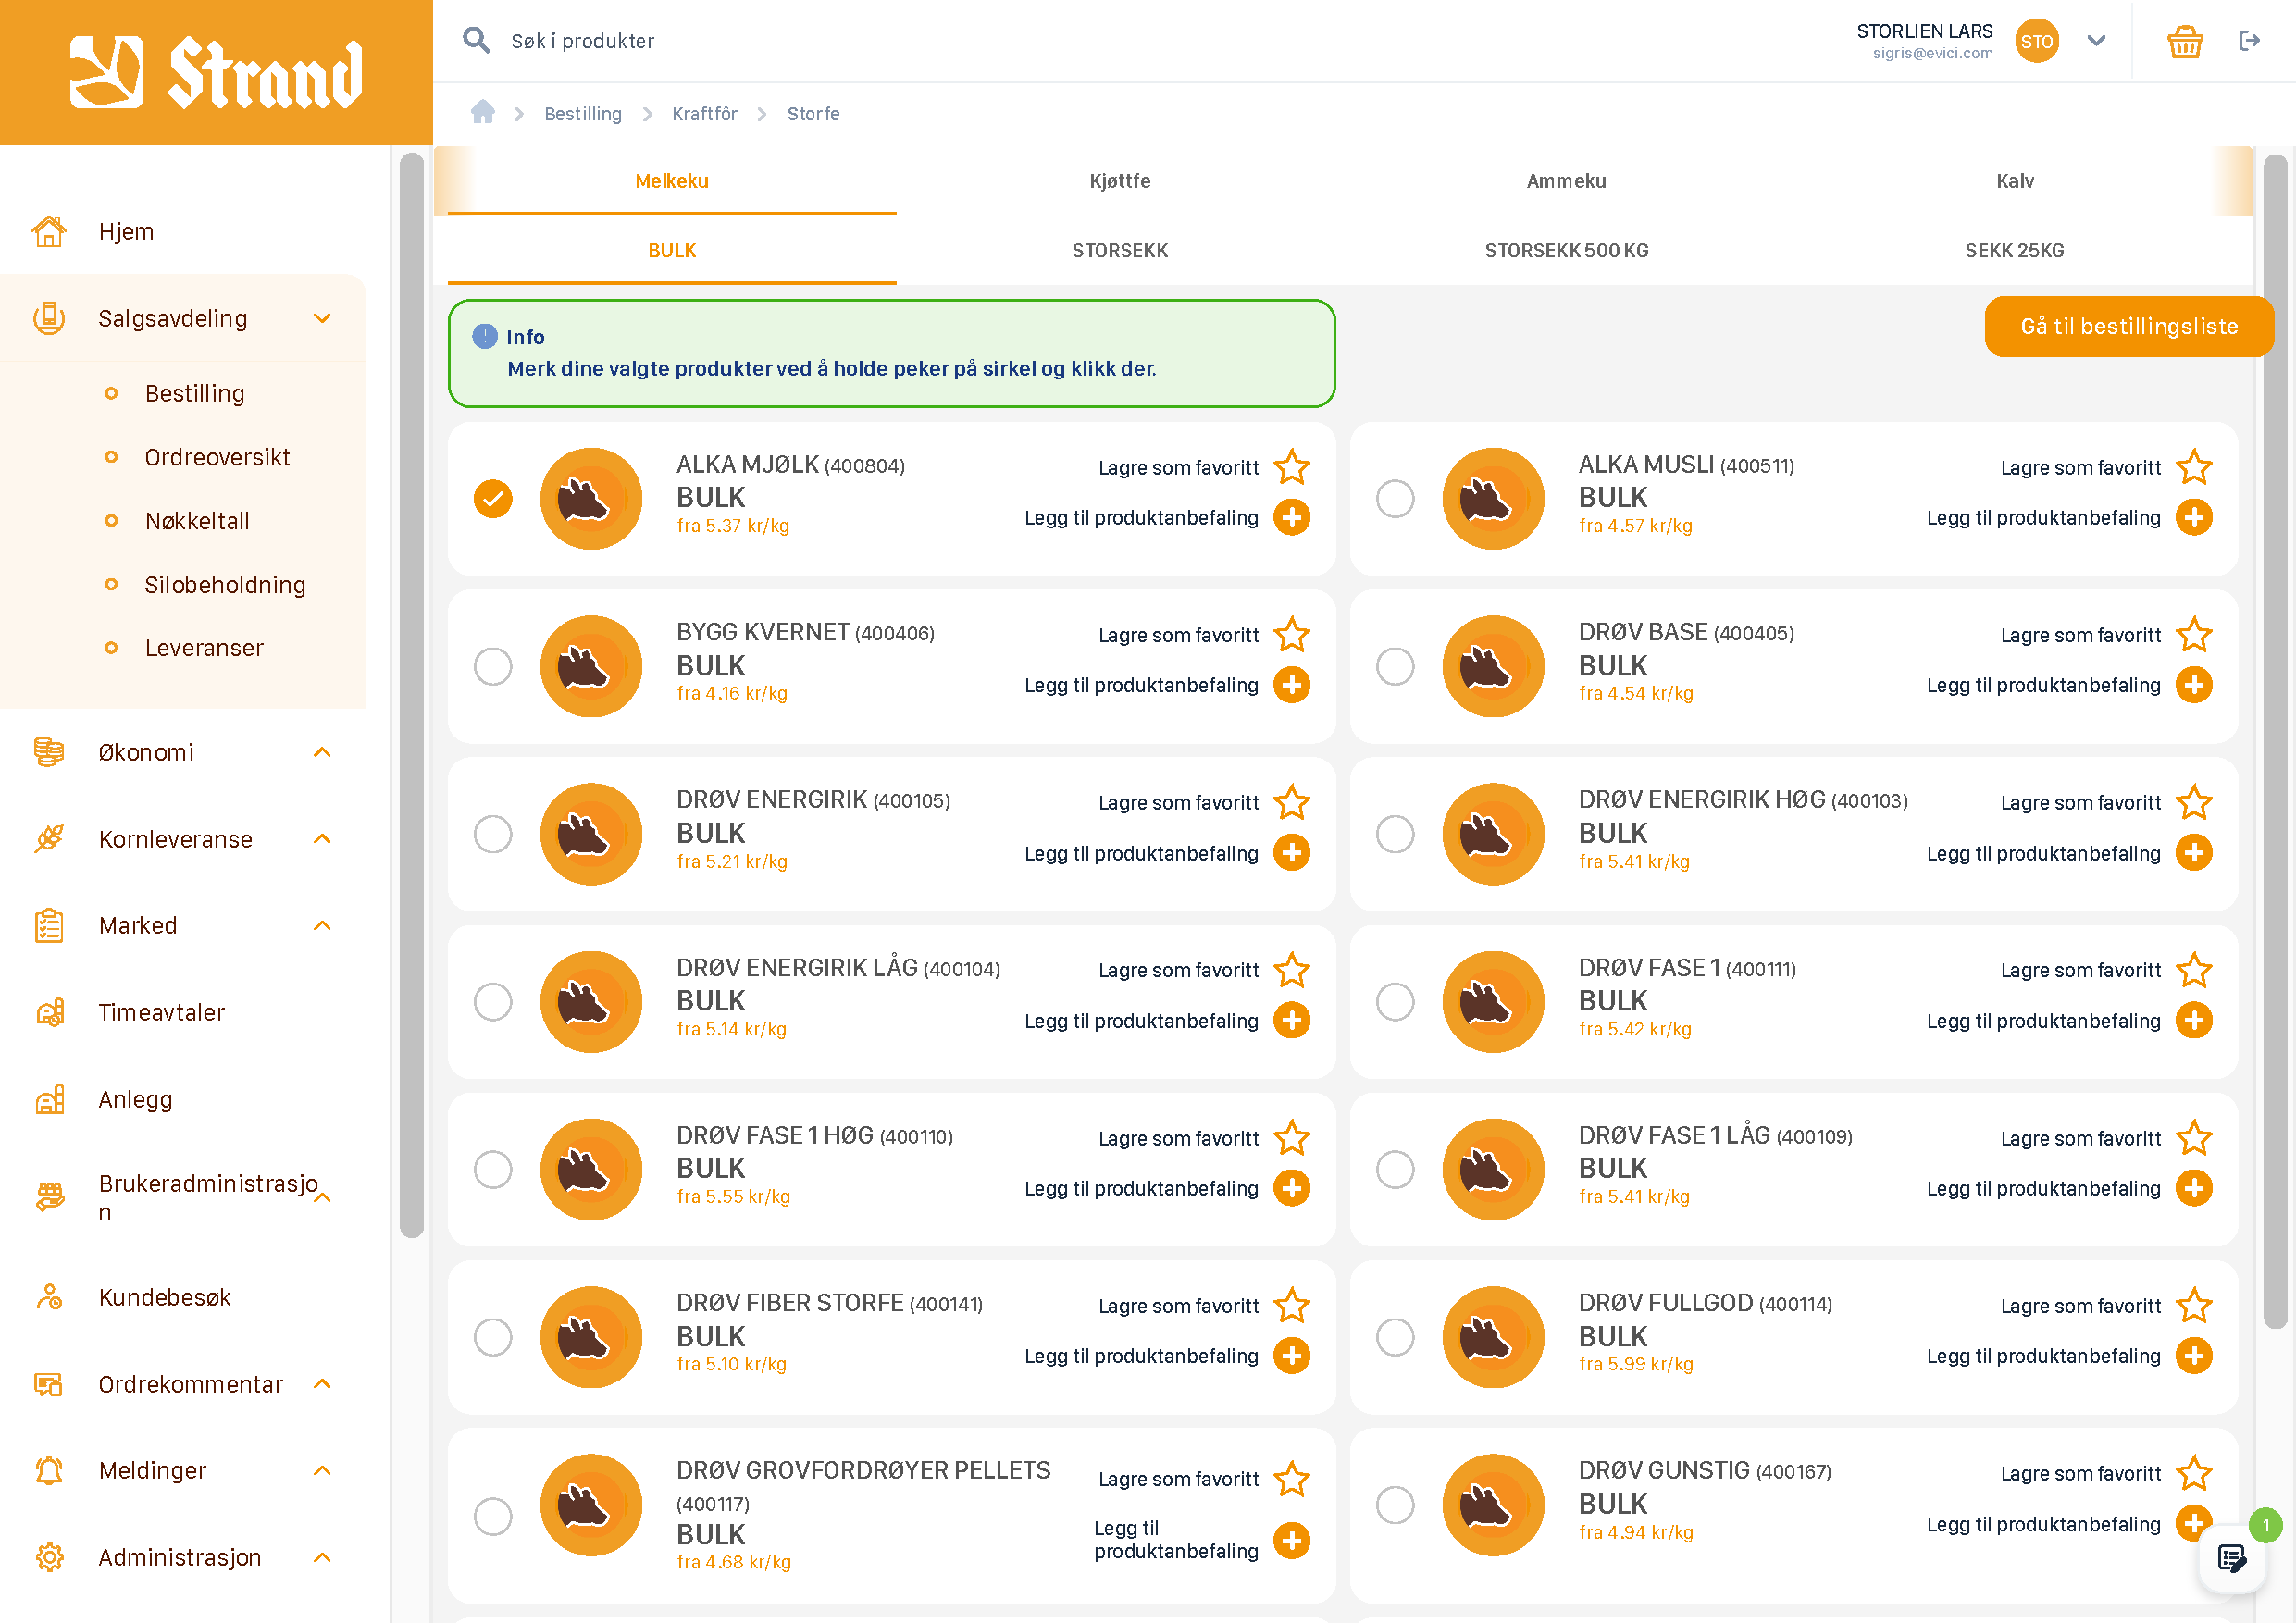
\includegraphics[width=\textwidth]{storfe-list.pdf}};

  \coordinate (SW) at (img.south west);
  \coordinate (SE) at (img.south east);
  \coordinate (NW) at (img.north west);

  \newcommand{\ip}[2]{($(SW) + {#1}*($(SE)-(SW)$) + {#2}*($(NW)-(SW)$)$)}

  \tikzset{
    badge/.style={
      circle,
      draw=strandOrange, fill=strandOrange,
      font=\bfseries\footnotesize\sffamily, text=white,
      inner sep=1.5pt, minimum size=14pt,
      drop shadow={shadow xshift=0.5pt, shadow yshift=-0.5pt}
    },
    arrow/.style={
      -{Stealth[length=5pt]},
      color=strandOrange,
      line width=0.9pt
    }
  }

  % ---- Badges (adjust coordinates after compiling) --------
  % Badge 10: TODO – point to the relevant click target
  \node[badge] (b10) at \ip{0.50}{0.50} {10};
  \draw[arrow] (b10) -- \ip{0.45}{0.50};

\end{tikzpicture}

\end{document}
